\section{RISK reglerne}
Hvert hold får udleveret 5 missionskort ved ankomst, missionerne kan være alt fra at bunde en sodavand over kidnapning af hyttebumser til at vinde udfordrerkappen. Derudover uddeles 5 nye missionskort hver morgen. Ved udførelse af en mission, skal en voksen være til stede for at godkende. På hvert kort er der et antal stjerner, som angiver hvor mange armeer, man får for udførelse af missionen. Armeerne er i dette tilfælde farvede knappenåle, som placeres i et land på RISK-kortet, som bliver hængt op i spisesalen og som ses på figur \ref{fig:RISK}. Der uddeleles desuden armeer til vinderne af natløb, krigsløb og taler. Regler:
\begin{itemize}
  \item Armeer må ikke placeres i nogens hjemland - disse er fredet
  \item Armeer kan frit placeres - der er ikke krav om at man skal støde op til et land for at angribe
  \item Det hold med flest armeer i et land ejer landet
  \item Man må ikke flytte en arme efter den er placeret
  \item Det er udelukkende de voksne der må sætte nåle i brættet
  \item Det er absolut forbudt at pille ved brikkerne, også når vektorerne ikke kigger
\end{itemize}
De sidste missioner skal være udført torsdag aften inden aftensmaden, og vinderen \Hashtag{verdensherskeren} kåres efter hovedretten - præmien er badges.

\begin{figure}[H]
\centering
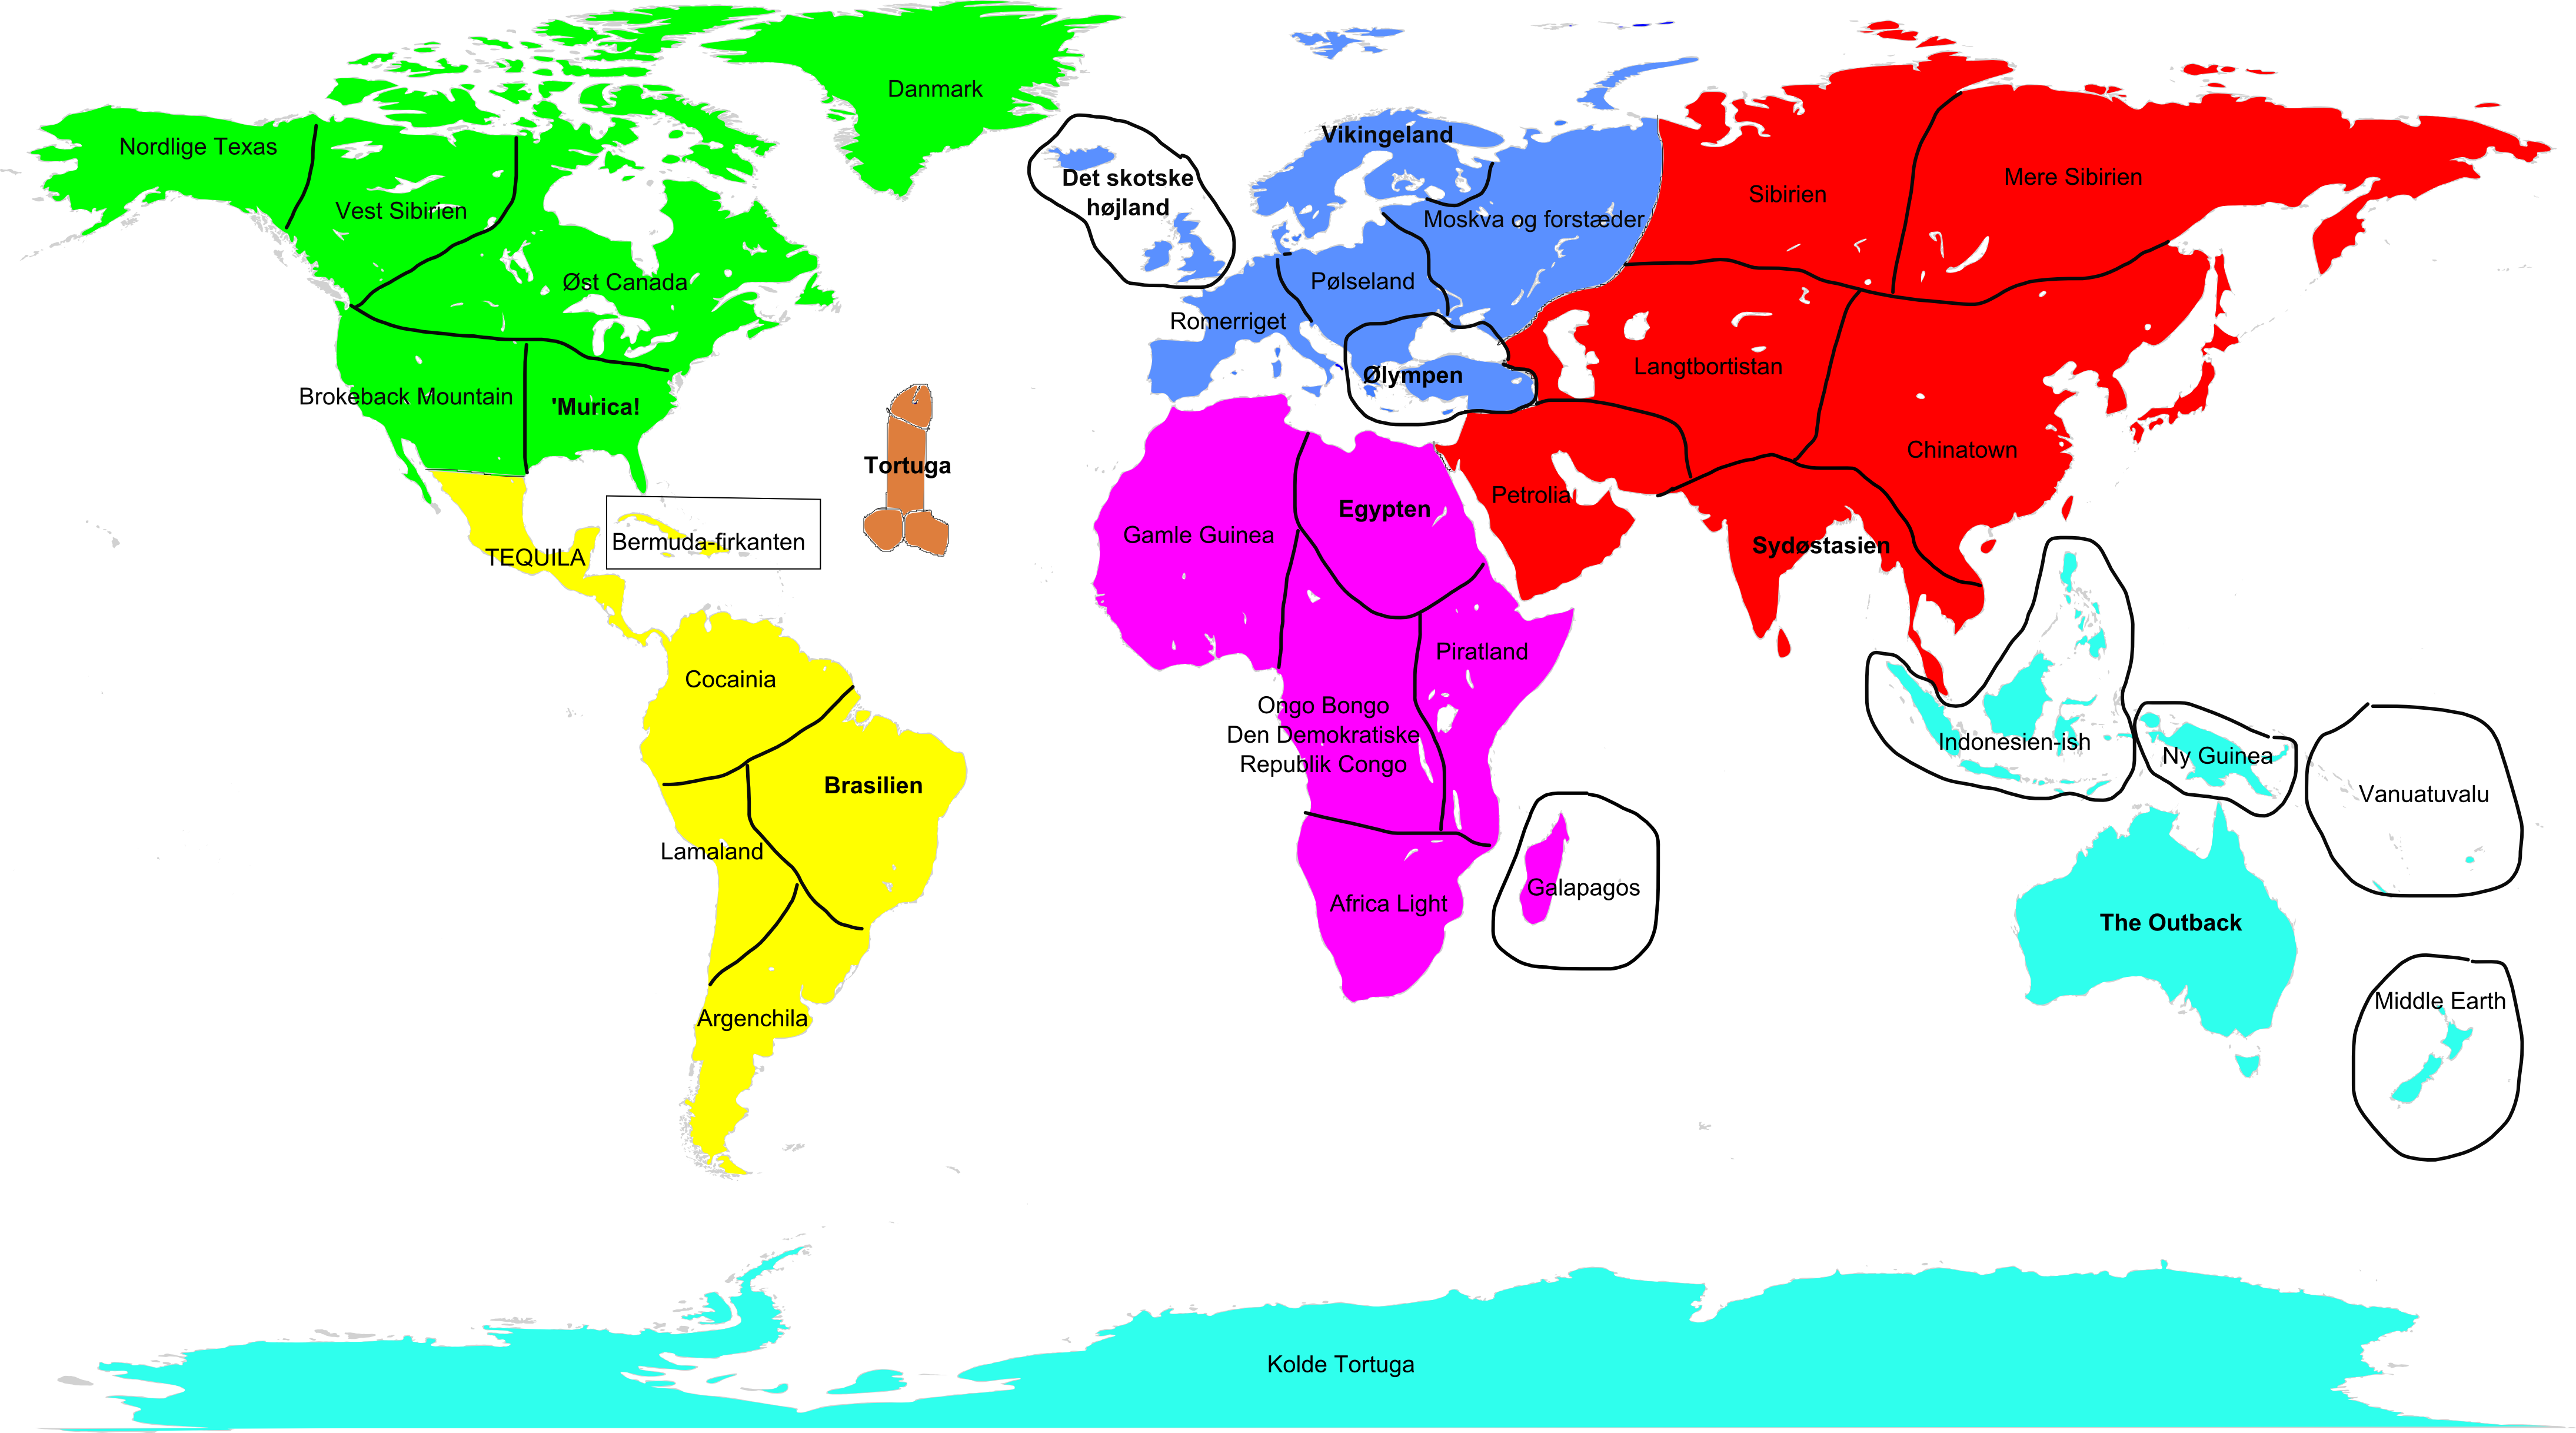
\includegraphics[width=\textwidth]{fig/Verdenskort.png}
\caption{RISK brættet}
\label{fig:RISK}
\end{figure}